\documentclass[xetex,mathserif,serif]{beamer}
\usepackage{polyglossia}
\setdefaultlanguage[babelshorthands=true]{russian}
\usepackage{minted}
\usepackage{tabu}

\useoutertheme{infolines}

\usepackage{fontspec}
\setmainfont{FreeSans}
\newfontfamily{\russianfonttt}{FreeSans}

\usepackage{forest}
\usetikzlibrary{arrows}

\setbeamertemplate{blocks}[rounded][shadow=false]
\setbeamercolor*{block title example}{fg=green!50!black,bg=green!20}
\setbeamercolor*{block body example}{fg=black,bg=green!10}

\setbeamercolor*{block title alerted}{fg=red!50!black,bg=red!20}
\setbeamercolor*{block body alerted}{fg=black,bg=red!10}

\tabulinesep=0.7mm

\title{Сложность алгоритмов}
\author[Юрий Литвинов]{Юрий Литвинов \newline \textcolor{gray}{\small\texttt{yurii.litvinov@gmail.com}}}

\date{21.09.2018}

\begin{document}
	
	\frame{\titlepage}
	
	\begin{frame}
		\frametitle{Сложность}
		\begin{itemize}
			\item Быстрее – не значит лучше!
			\begin{itemize}
				\item Время работы программиста может быть дороже времени работы программы
%				\item Но может быть и наоборот, если программа часто используется
			\end{itemize}                                                     
			\item Сложность
			\begin{itemize}
				\item Вычислительная (время работы)
				\item Емкостная (объём потребляемой памяти)
%				\item Они взаимосвязаны
			\end{itemize}
			\item Вычислительную сложность непонятно, как измерять
			\begin{itemize}
				\item Зависит от машины, на которой считаем
				\item Зависит от объёма входных данных
%				\item Зависит от самих входных данных
			\end{itemize}
		\end{itemize}
	\end{frame}

	\begin{frame}
		\frametitle{Асимптотическая сложность}
		\begin{itemize}
			\item O-символика
			\begin{center}
				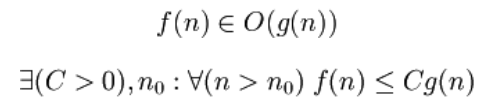
\includegraphics[width=0.8\textwidth]{complexity-o-notation.png}
			\end{center}
			\item То есть “f принадлежит классу функций O(g), если начиная с некоторого $n_0$ она ограничена сверху функцией g с точностью до некоторого наперёд заданного множителя”
			\item Или ещё более то есть – “f растёт не быстрее g”
		\end{itemize}
	\end{frame}

	\begin{frame}
		\frametitle{Пример}
		\begin{center}
			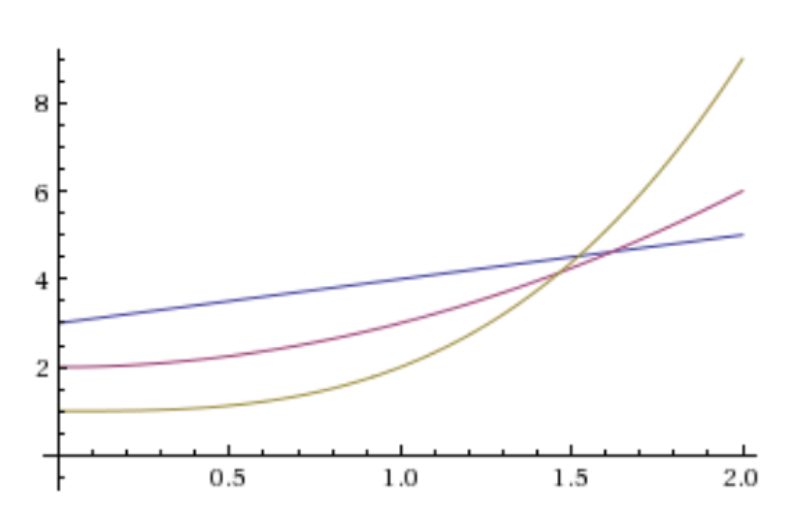
\includegraphics[width=0.8\textwidth]{example.png}
		\end{center}
	\end{frame}

	\begin{frame}
		\frametitle{Правила вычисления трудоёмкости}
		\begin{itemize}
			\item Оператор S1 выполняется за время T1(n), имеющее порядок O(f(n)), оператор S2 – за время T2(n), имеющее порядок O(g(n)), тогда S1; S2 выполняется за время O(max(f(n), g(n)))
			\begin{itemize}
				\item Следствие: O(n2 + n) = O(n2)
			\end{itemize}
			\item Если S1 внутри себя порядка O(f(n)) раз вызывает S2, то итоговая трудоёмкость равна O(f(n) * g(n))
			\begin{itemize}
				\item Это правило позволяет анализировать циклы
			\end{itemize}	
		\end{itemize}
	\end{frame}
	
        \begin{frame}[fragile]
		\frametitle{Пример: пузырёк}        
		\begin{footnotesize}
			\begin{minted}{cpp}
for (int i = 0; i < n; ++i)                  // O((n - 1) + … + 1) = O(n(n-1)/2) = O(n2)
    for (int j = n; j > i; --j)                  // O((n - i) * 1) = O(n - i)
        if (a[j - 1] > a[j])                      // O(1)
             swap(a[j - 1], a[j]);             // O(1)
			\end{minted}
		\end{footnotesize}

		\begin{itemize}
			\item Бывают сортировки за O(n*log(n))
			\item Бывает сортировка подсчётом, за O(n)
			\item Это важно, $log(2, 1000000) ~ 20$
			\begin{itemize}
				\item Обратите внимание, $O(log(2, n)) = O(ln(n))$
			\end{itemize}
		\end{itemize}
	\end{frame}

	\begin{frame}[fragile]
		\frametitle{Анализ рекурсивных алгоритмов}
		\begin{footnotesize}
			\begin{minted}{cpp}
int recFact(int a) {
      if (a <= 1)
              return 1;
      else
              return a * recFact(a - 1);
}
			\end{minted}
		\end{footnotesize}
		\begin{itemize}
			\item $T(n) = c + T(n-1)$ при $n > 1$, и $d$, при $n <= 1$
			\item $T(n) = c + T(n-1) = 2c + T(n-2) = ... = i*c + T(n-i) = ... = (n-1)*c + T(1) = (n-1)*c+d$
		\end{itemize}
	\end{frame}
        
	\begin{frame}
		\frametitle{Числа Фибоначчи}
		\begin{itemize}
			\item $F_n = F_n-2 + F_n-1, F_0 = 1, F_1 = 1$
			\item F = 1, 1, 2, 3, 5, 8, 13, 21, …
			\item Рекурсивное решение – ?
			\item Итеративное решение – ?
			\item Решение за O(log(n)):
			\begin{center}
				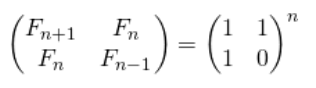
\includegraphics[width=0.8\textwidth]{fibonacci_log_n.png}
			\end{center}
			\item Формула Бине:
			\begin{center}
				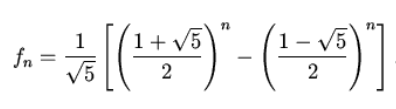
\includegraphics[width=0.8\textwidth]{fibonacci_bine.png}
			\end{center}
		\end{itemize}
	\end{frame}

	\begin{frame}
		\frametitle{Пример времён вычисления в зависимости от трудоёмкости алгоритма}
			\begin{center}
				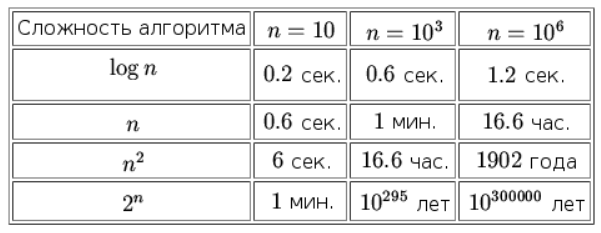
\includegraphics[width=0.8\textwidth]{complexity-table.png}
			\end{center}		
	\end{frame}

\end{document}

